\subsection{Done Задание 5. Разрешение во времени простых и сложных сигналов при
согласованной фильтрации.}

Проанализируем разрешение сигналов во времени при использовании согласованного фильтра.
Качественно можно считать, что сигналы разрешены, если их максимумы
отстоят не менее, чем на величину длительности сигнала.

Отметим, что если величина временной задержки больше длительности сигнала, то входные сигналы разнесены по времени, 
и уже считаются разрешенными. Поэтому, в дальнейшем будем рассматривать задержки величиной
до длительности сигнала.

\subsubsection{Прямоугольный видеоимпульс}
Проводились измерения при значениях длительности сигналов $T = 10, 20, 40$ мс. Пример суперпозиции сигналов, а также
выход с фильтра приведены на рис. \ref{fig:task5_1_10_15}.
\begin{figure}[H]
    \centering
    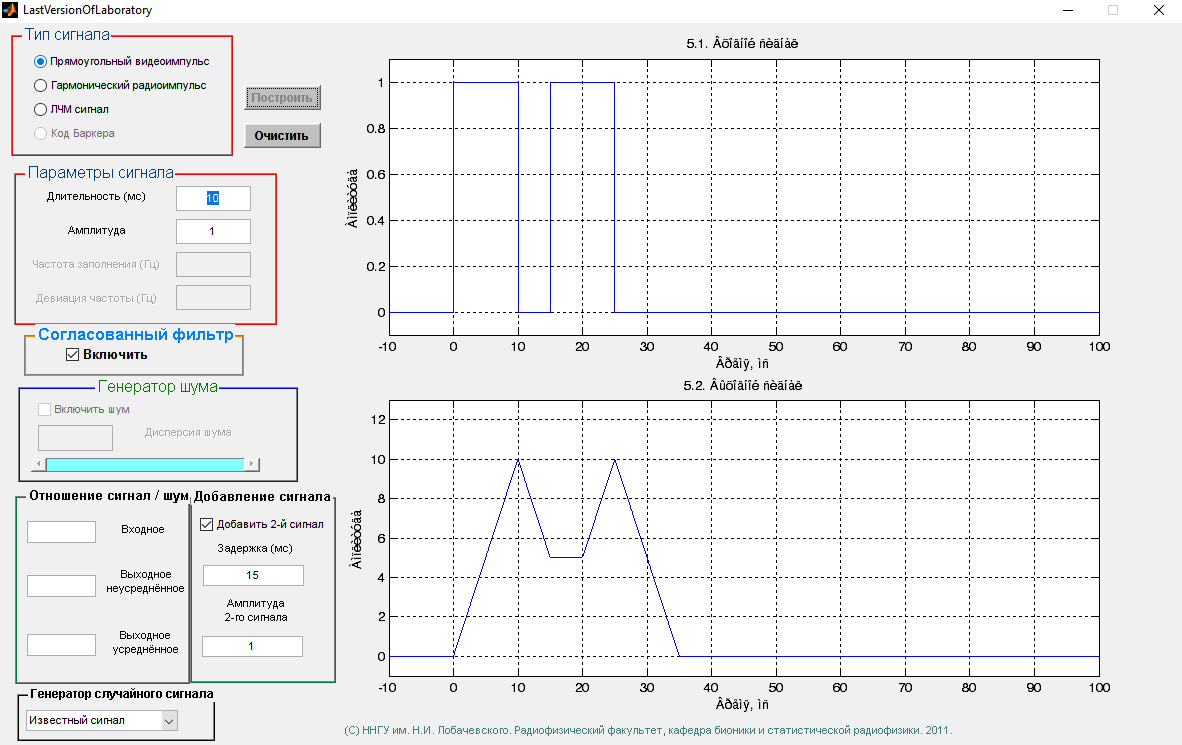
\includegraphics[width=0.7\linewidth]{imgs/task5/t5s1_dur10_del15.png}
    \caption{Прямоугольный видеоимпульс. Длительность 10 мс, задержка 15 мс}
    \label{fig:task5_1_10_15}
\end{figure}
При длительности импульса 10 мс, качественно, сигналы стали различимы при задержке в 11 мс - появились явные разделенные
пики, по которым можно различить два сигнала. Однако при задержке в 11 мс, как было скачано раньше, наступает разделение
сигналов на входе. 

Если задержка между сигналами равна длительности первого сигнала, то два входных прямоугольных видеоимпульса
сливаются в один, длительность которого становится равной 20 мс, и на входе фильтра эти сигналы не разрешены, и на
выходе согласованного фильтра наблюдается только один выходной сигнал - сигналы не разрешены.

Использование согласованной фильтрации не позволяет разрешить два прямоугольных видеоимпульса подданных неразрешенными на вход фильтра. 



\subsubsection{ЛЧМ сигнал}
Далее исследовался ЛЧМ сигнал с частотой заполнения $f=3000$ Гц, девиацией $\Delta f = 200, 400, 800$ Гц, одинаковыми амплитудами, и
длительностью $T=10, 20, 40$ мс. ЛЧМ сигналы это сложные сигналы, чья база $B$ много больше единицы: $B = T \cdot \Delta f \in (2,32)$
\begin{figure}[H]
    \centering
    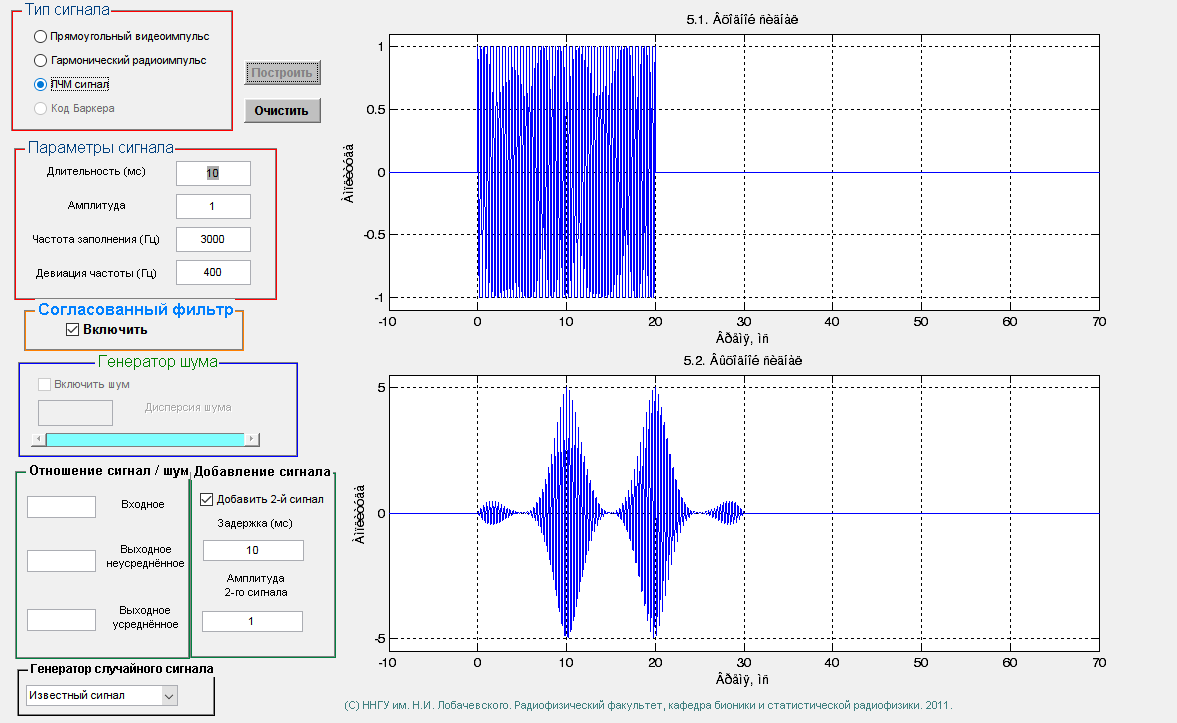
\includegraphics[width=0.6\linewidth]{imgs/task5/lfm_dev400/t5s21_dur10_del10_dev400.png}
    \caption{ЛЧМ сигнал, $T=10$ мс, $\Delta f=400$ Гц, $\Delta t=10$ мс}
    \label{fig:t5s21_dur10_del10_dev400}
\end{figure}

Рассмотрим сигналы с одинаковой амплитудой и длительностью.
На рис. \ref{fig:t5s21_dur10_del10_dev400} приведены осциллограммы входного и выходного сигнала, длительностью
$T=10$ мс, $\Delta f=400$ Гц, значение задержки $\Delta t = 10$ мс. На входе сигналы не разрешены - они сливаются в один
сигнал длительностью 20 мс, однако на выходе согласованного фильтра наблюдается два разнесенных по времени пика.

Так происходит, потому  что эффеткивная длительность сигнала уменьшается в $B$ раз при прохождении согласованного фильтра. Таким образом,
эффективная длительность каждого сигнала на выходе:
\begin{equation}
    T_{eff} = \frac{T}{B} = \frac{1}{\Delta F}=\frac{10}{4} = 2.5 \text{мс}
    \label{eq:effective_dur}
\end{equation}

В случае, когда задержка меньше длительности, например $\Delta t = 5$ мс, на входе сигналы перекрываются
(см. рис. \ref{fig:t5s21_dur10_del5_dev400}). При этом на выходе согласованного фильтра все также наблюдаются два
отчетливо разнесенных отклика.
\begin{figure}[H]
    \centering
    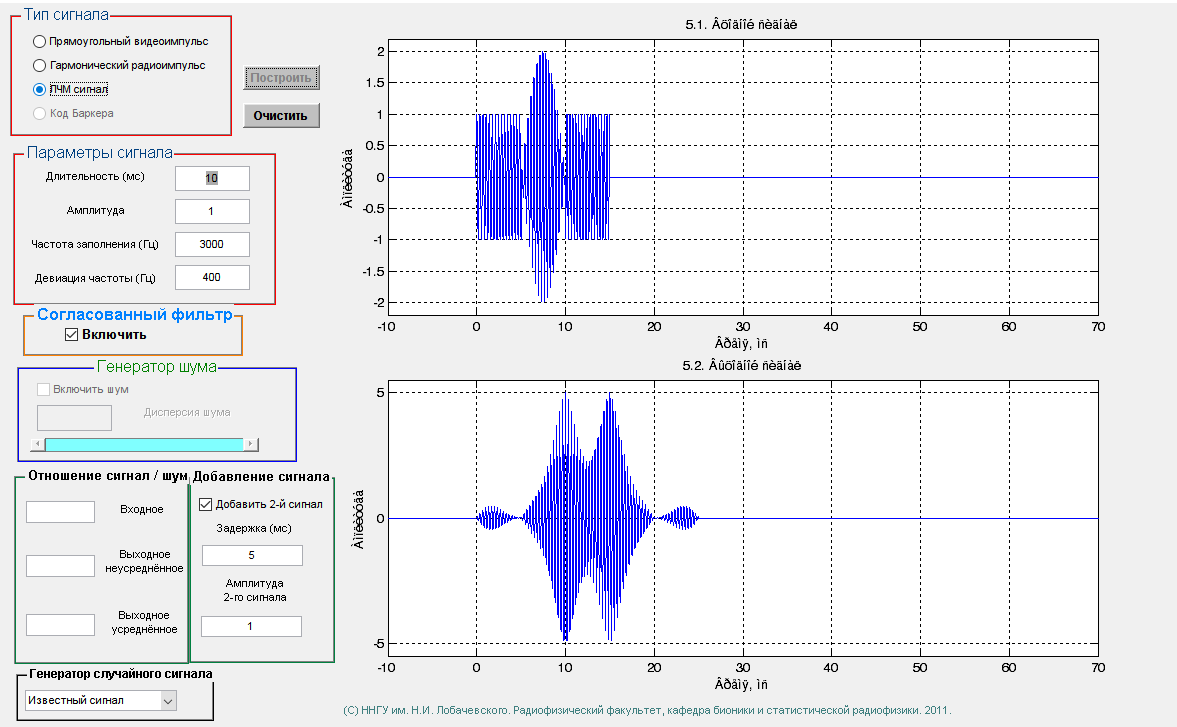
\includegraphics[width=0.6\linewidth]{imgs/task5/lfm_dev400/t5s21_dur10_del5_dev400.png}
    \caption{ЛЧМ сигнал, $T=10$ мс, $\Delta f=400$ Гц, $\Delta t=5$ мс}
    \label{fig:t5s21_dur10_del5_dev400}
\end{figure}

Для сигнала в $T=10$ мс, $\Delta f=400$ Гц, значение задержки $\Delta t$, при котором становятся различимы сигналы,
составляет $\Delta t=6$ мс.

Далее варьировались параметры сигналов и определялось минимальное значение временной задержки сигналов.
По результатам измерений была составлена следующая таблица, в которой указаны пороговые значения задержки в мс, при
которых сигналы становились различимыми:
\begin{table}[H]
    \centering
    \begin{tabular}{|x{2.0cm}|l|l|l|}
    \hline
    \diag{.1em}{2.0cm}{$\Delta f$, Гц }{T,мс}  & 10 & 20 & 30 \\ \hline
    200 &  6  &  6  &  7  \\ \hline
    400 &  3  &  3.05  &  3.05  \\ \hline
    800 &  1.2  &  1.1  &  1.1  \\
    \hline 
    \end{tabular}
\end{table}
Из полученных данных видно, что увеличение длительности сигнала слабо практически не влияет на разрешающую способность,
в то время как величина девиации напрямую влияет на разрешающую способность - эффективная длительность сигнала на выходе $T_{eff} =
\frac{1}{\Delta f}$. Укорачивая длительность сигналов, они разносятся на выходе, повышая разрешающую способность.

Видно преимущество сложных сигналов - даже слившиеся или перектрытые сигналы можно разрешить,
используя согласованный фильтр.

Также рассмотрим сигналы с разной амплитудой. Пусть амплитуда задержанного сигнала меньше основного в $\sim 6$ раз.
Длительность $T=10$ мс, $\Delta f=400$ Гц, значение задержки $\Delta t = 10$ мс (см. рис. \ref{fig:t5s21_dur10_del10_dev400_amp6}).
\begin{figure}[H]
    \centering
    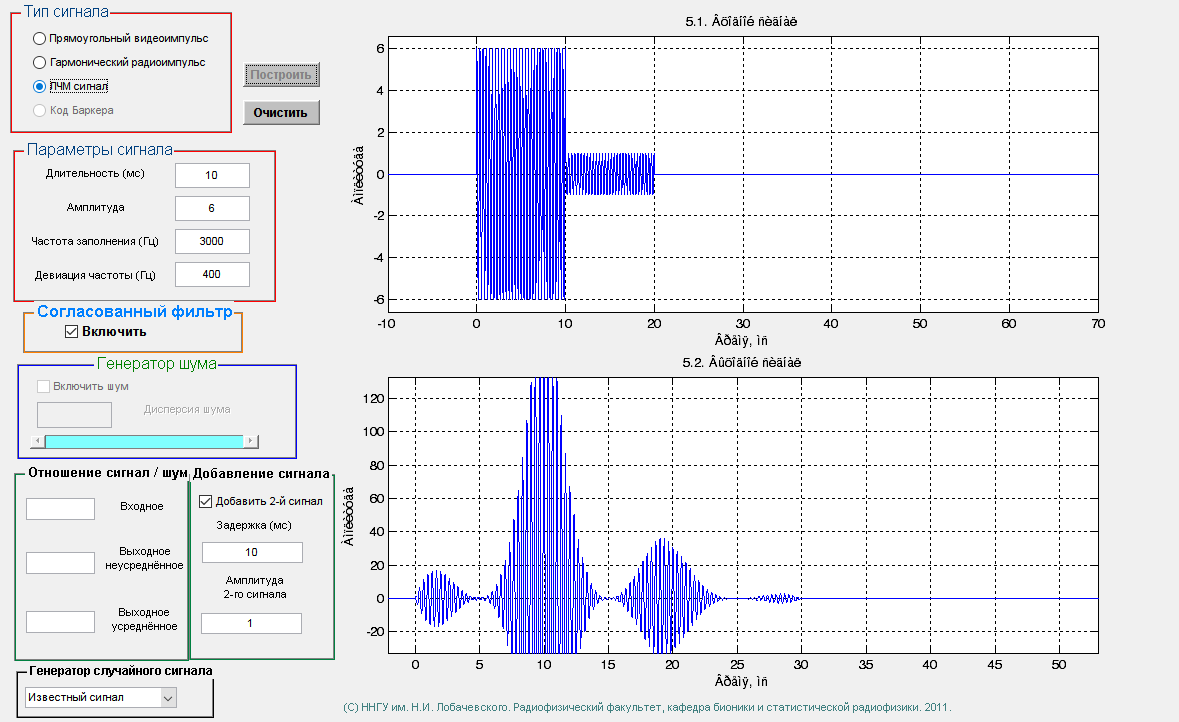
\includegraphics[width=0.6\linewidth]{imgs/task5/lfm_dev400/6amp/t5s21_dur10_del10_dev400_amp6.png}
    \caption{ЛЧМ сигнал, $T=10$ мс, $\Delta f=400$ Гц, $\Delta t=10$ мс, $A_1 = 6A_2$}
    \label{fig:t5s21_dur10_del10_dev400_amp6}
\end{figure}
На выходе фильтра наблюдается два отклика, разнесенные по времени. Таким образом, сигналы разрешены и на входе (по
амплитуде), и на выходе (по времени). Однако стоит отметить, что в данной ситуации отклик второго испульса накладывается
на побочный лепесток первичного импульса, и возможна ситуация, при которой сигналы будет невозможно разрешить.

\paragraph{Вывод}
Используя сложные сигналы, можно обеспечить необходимую разрешающую способность, поскольку проходя через согласованный
фильтр, эффективная длительсноть сигнала сокращается в $B$ раз, что бессмысленно в случае с простыми сигналами, которые
невозможно различить при задержке меньше длительности.
